\documentclass{beamer}

% german content
\usepackage[ngerman]{babel}

% bibliography
\usepackage[
  backend=biber,
  style=authoryear,
  citestyle=authoryear,
  autocite=footnote
]{biblatex}
\addbibresource{bibliography.bib}

% images
\usepackage{graphicx}
\graphicspath{ {./images/} }

\title{Ahnenforschung mit DNA}
\subtitle{}
\author{Jonathan Neidel, 573619 \and github.com/jneidel/Ahnenforschung-mit-DNA}
\date{Juni 2021}
\institute{HTW Berlin, Angewandte Informatik, Datenschutz und Datensicherheit}
\logo{
\includegraphics[width=1cm]{logo}}

% theme + color theme
\usetheme{Szeged}
\usecolortheme{whale}
% see: https://deic-web.uab.cat/~iblanes/beamer_gallery/index.html
\setbeamerfont{caption}{size=\Tiny}

\begin{document}
\frame{\titlepage}

\section{Ahnenforschung}
\begin{frame}
  \begin{center}
    {\Huge Was ist Ahnenforschung?}
  \end{center}
\end{frame}

\begin{frame}
  \frametitle{Definition DNA Ahnenforschung}

  \begin{itemize}
    \item erforschen biologischer Herkunft
      \begin{itemize}
        \item Familiengeschichte basierend auf schriftlichen Aufzeichnungen
        \item DNA gestüzte Auswertung
      \end{itemize}
  \end{itemize}
\end{frame}

\begin{frame}
  \frametitle{Test Kits}

  \centering
    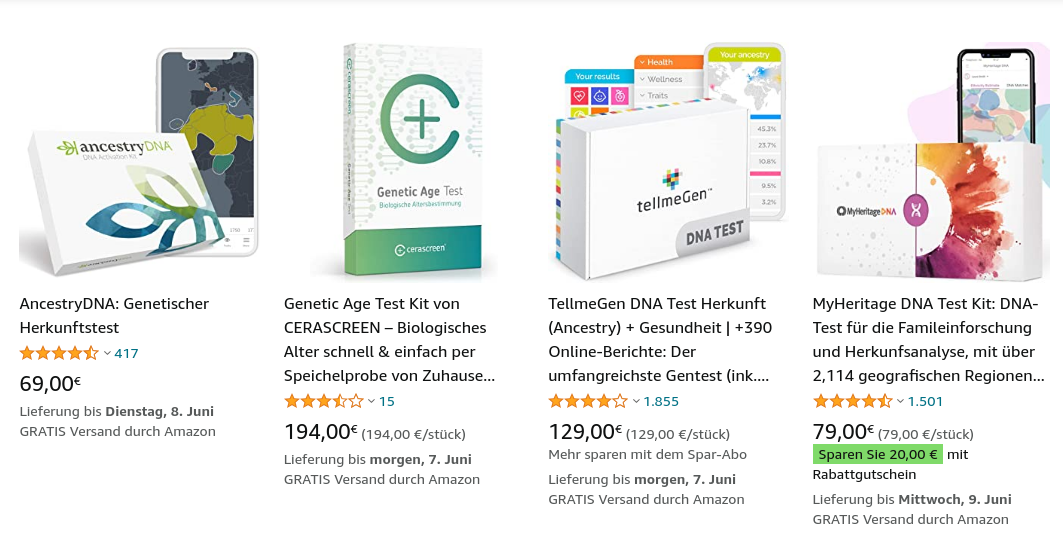
\includegraphics[scale=0.3]{test-kits}
\end{frame}

\begin{frame}[allowframebreaks]
  \frametitle{Services}

  \begin{enumerate}
    \item Abstammung feststellen
      \begin{itemize}
        \item biogeographische Herkunftsanalyse
        \item 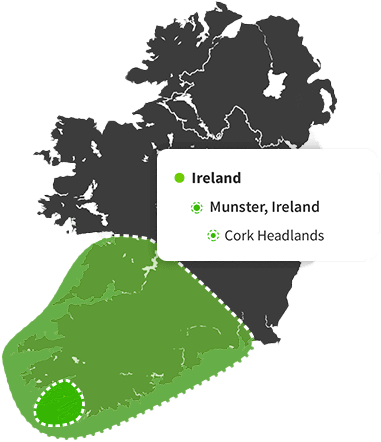
\includegraphics[scale=0.2]{dna-regions}
        \item "Lang gesuchte oder bisher unbekannte Verwandte [identifizieren]"\autocite{ancestryBlog}
        \item Legal\autocite{genDG2}
      \end{itemize}
    \break
    \item Gesundheitliche Auswertung
      \begin{itemize}
        \item Veranlagungen für Krankheiten
        \item Illegal\autocite{genDG7}
      \end{itemize}
  \end{enumerate}
\end{frame}

\begin{frame}
  \frametitle{Zielgruppe}

  \begin{itemize}
    \item USA: Einwandernation
    \item Deutschland: zunehmende Migration und globale Wanderungsbewegungen
  \end{itemize}
\end{frame}

\section{Anbieter}
\begin{frame}
  \begin{center}
    {\Huge Wer sind die Anbieter?}
  \end{center}
\end{frame}

\begin{frame}
  \frametitle{Globale Marktführer und deren Besitzer}

  Ancestry
  \begin{itemize}
    \item majority stake von Blackstone aufgekauft\autocite{Ancwiki}
      \begin{itemize}
        \item \$650 Mrd. AUM\autocite{blackstone}
      \end{itemize}
  \end{itemize}

  23andMe
  \begin{itemize}
    \item Google\autocite{23wiki}
      \begin{itemize}
        \item früher Investor
        \item CEO Ex-Frau von Google Mitgründer
    \end{itemize}
    \item 60 Investoren, u.a.\autocite{23owners}
      \begin{itemize}
        \item Virgin Group
        \item GlaxoSmithKline (Pharma)
      \end{itemize}
  \end{itemize}
\end{frame}

\begin{frame}[allowframebreaks]
  \frametitle{DNA Testing Market}
  Datensätze:\autocite{ancestryGER}
  \begin{itemize}
    \item Ancestry: 10 Mio.
    \item 23andMe: 5 Mio.
  \end{itemize}

  \break

  Winner Take Most Market

  \bigskip

  Netzwerkeffekt ... Produktnutzen steigt mit Anzahl der Nutzer

  \medskip

  \begin{itemize}
    \item "Lang gesuchte oder bisher unbekannte Verwandte [identifizieren]"\autocite{ancestryBlog}
  \end{itemize}
\end{frame}

\begin{frame}
  \frametitle{Einnahmequellen von Ancestry\autocite{ancestryGER}}

  \begin{enumerate}
    \item Auskunftserteilung für Verbraucher
    \item Beschaffung der DNA für eigene kommerzielle Zwecke
  \end{enumerate}
\end{frame}

\section{Datenhandhabung}
\begin{frame}
  \begin{center}
    {\Huge Was machen die Anbieter mit den Daten?}
  \end{center}
\end{frame}

\begin{frame}
  \frametitle{Datenschutz: Teilen Genetischer Daten mit Dritten}

  Ancestry:
  \begin{itemize}
    \item Opt-in
    \item wahrscheinlich 80\% der Nutzer stimmen zu\autocite{bbc}
    \item Geteilt mit:
      ``akademische Einrichtungen sowie Non-Profit-Organisationen, gewinnorientierte Unternehmen und Regierungsbehörden''\autocite{bigbro}
  \end{itemize}

  Rest der US Branche:
  \begin{itemize}
    \item 78\% teilen genetische Daten mindestens in anonymisierter bzw. aggregierter Form mit Dritten\autocite{privacyCompare}
  \end{itemize}
\end{frame}

\begin{frame}
  \frametitle{Datenschutz: Einschätzung}

  Experte:
  \begin{itemize}
    \item als Einwilligungserklärung zu unbestimmt $\Rightarrow$ unwirksam\autocite{ancestryGER}
  \end{itemize}

  \medskip

  Meine:
  \begin{itemize}
    \item wenn ehrlich andere Formulierung als: "Der Schutz ihrer Daten ist uns sehr wichtig."\autocite{ancestryGER}
    \item vgl. Googles ``We do not sell your personal information [..]''\autocite{effGoogle}
  \end{itemize}
\end{frame}

\begin{frame}
  \frametitle{Datenschutz: Gendiagnostikgesetz}

``Es dürfen nur die zur Klärung der Abstammung erforderlichen Untersuchungen an
der genetischen Probe vorgenommen werden. Feststellungen über andere Tatsachen
  dürfen nicht getroffen werden.''\autocite{genDG17}

  \medskip

  \begin{itemize}
    \item Forschungsprivileg?
    \item Nein: nicht für rein kommerzielle Unterfangen (Pharmaindustrie)\autocite{ancestryGER}
  \end{itemize}
\end{frame}

\begin{frame}
  \frametitle{Publiziertes Beispiel\autocite{bigbro}}

  \begin{itemize}
    \item 23andMe (halb so großer Datenbestand)
    \item \$300 Mio. Kooperationsvertrag mit Pharmakonzern zur Datennutzung
  \end{itemize}
\end{frame}

\begin{frame}
  \frametitle{Einordnung der Einnahmequellen}

``Das Geschäftsmodell dieser Anbieter ist nicht die Ahnenforschung, sondern es
geht um das ganz große Geld mit den Gendaten [..]''\autocite{bigbro}
\end{frame}

\section{Folgerungen}
\begin{frame}
  \begin{center}
    {\Huge Was bedeutet das für den Nutzer?}
  \end{center}
\end{frame}

\begin{frame}
  \frametitle{Abzocke\autocite{bigbro}}

  \begin{itemize}
    \item ``[..] Tatsächlich werden die Betroffenen abgezockt.''
    \item vgl. Google, Facebook und Co. mit Internetdaten
    \item Kompensation `nur' Auswertungsergebnisse
    \item Keine Gewinnbeteiligung als vermeintliche `Dateneigentümer'
  \end{itemize}
\end{frame}

\begin{frame}
  \frametitle{Sensitivität der Daten}

  \begin{itemize}
    \item dauerhaft persönlich identifizierend
    \item mit Famile geteilt:
    \item 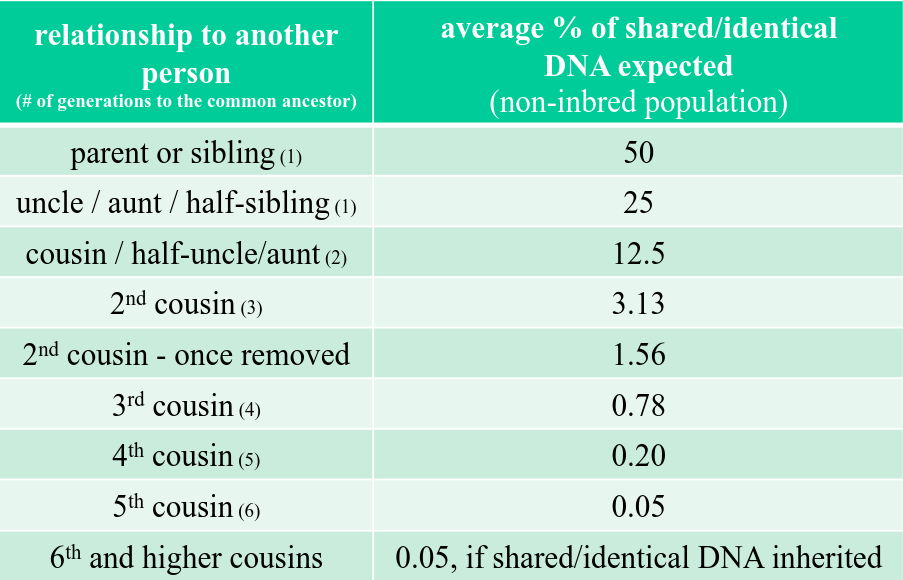
\includegraphics[scale=0.18]{shared-dna}\autocite{tedx}
    \item vlg. Grundrecht auf Datenschutz von Dritten\autocite{ancestryGER}
  \end{itemize}
\end{frame}

\section{Fazit}
\begin{frame}[allowframebreaks]
  \frametitle{Fazit}

  \begin{center}
    {\Huge Fazit}
  \end{center}

  \break

  ``[es] wird allen VerbraucherInnen geraten, auf die Inanspruchnahme dieses
  Angebots sowie von vergleichbaren Angeboten zu verzichten. Sie entledigen sich
  damit nicht nur ihrer eigenen genetischen Selbstbestimmung, sondern berauben
  auch ihre biologischen Verwandten dieses Rechtes.''\autocite{ancestryGER}
\end{frame}

\begin{frame}
  \frametitle{Diskussion}

  \begin{itemize}
    \item Ist es im Kapitalismus nicht unvermeidlich, dass bezüglich des Datenschutzes
gegen das Interesse der Nutzer gearbeitet wird?
  \end{itemize}
\end{frame}

\begin{frame}[allowframebreaks]
  \frametitle{Bibliography}
  \printbibliography
\end{frame}

\end{document}
